\documentclass[tikz,border=2pt]{standalone}
\usepackage{amsmath,amssymb}
\usetikzlibrary{arrows.meta}
\begin{document}
% Nonnegative loading and no rip-off bound the premium: E[X] <= Pi(X) <= ess sup X.
% For deterministic X = 10 the band shrinks to the point 10, so Pi(X) = 1.2 E[X] = 12 violates no rip-off.
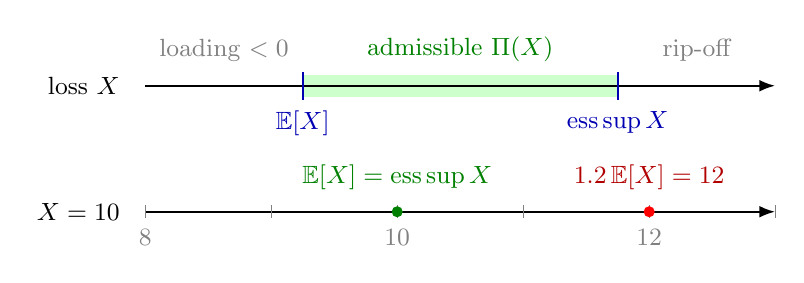
\begin{tikzpicture}[font=\small, >={Latex[length=2mm]}]
  % general loss
  \node[anchor=east] at (-0.2,0) {loss $X$};
  \fill[green!20] (2,-0.14) rectangle (6,0.14);
  \draw[->, thick] (0,0) -- (8,0);
  \draw[blue!70!black, thick] (2,-0.18) -- (2,0.18);
  \draw[blue!70!black, thick] (6,-0.18) -- (6,0.18);
  \node[blue!70!black, anchor=north] at (2,-0.2) {$\mathbb E[X]$};
  \node[blue!70!black, anchor=north] at (6,-0.2) {$\operatorname{ess\,sup}X$};
  \node[green!50!black, anchor=south] at (4,0.18) {admissible $\Pi(X)$};
  \node[gray, anchor=south] at (1,0.18) {loading $<0$};
  \node[gray, anchor=south] at (7,0.18) {rip-off};
  % deterministic loss X = 10, axis value v at x = 1.6(v-8)
  \node[anchor=east] at (-0.2,-1.6) {$X=10$};
  \draw[->, thick] (0,-1.6) -- (8,-1.6);
  \foreach \v in {8,9,10,11,12,13} \draw[gray] (1.6*\v-12.8,-1.68) -- (1.6*\v-12.8,-1.52);
  \foreach \v in {8,10,12} \node[gray, anchor=north] at (1.6*\v-12.8,-1.7) {$\v$};
  \fill[green!50!black] (3.2,-1.6) circle (2pt);
  \node[green!50!black, anchor=south] at (3.2,-1.45) {$\mathbb E[X]=\operatorname{ess\,sup}X$};
  \fill[red] (6.4,-1.6) circle (2pt);
  \node[red!70!black, anchor=south] at (6.4,-1.45) {$1.2\,\mathbb E[X]=12$};
\end{tikzpicture}
\end{document}
